\documentclass[acmsmall,review,anonymous]{acmart}

\usepackage{graphicx}
\usepackage{subfig}
\usepackage{textcomp}
\usepackage{multirow}
\usepackage{xcolor}
\usepackage{url}
\usepackage{tikz}
\usetikzlibrary{positioning,arrows.meta,shapes.geometric,fit,calc}
\usepackage{booktabs}
\usepackage[compact]{titlesec}
\titlespacing{\section}{0pt}{1.0\baselineskip}{0.4\baselineskip}
\titlespacing{\subsection}{0pt}{0.7\baselineskip}{0.3\baselineskip}
\titlespacing{\subsubsection}{0pt}{0.5\baselineskip}{0.2\baselineskip}
\usepackage{pifont}
\newtheorem{definition}{Definition}
\newtheorem{observation}{Observation}
\newtheorem{property}{Property}
\setcopyright{none}
\settopmatter{printacmref=false, printccs=true, printfolios=true}

% ---------- acronyms ----------
\newcommand{\pdm}{PDM}
\newcommand{\msbd}{MSBD}
\newcommand{\ctpr}{CTPR}
\newcommand{\cic}{CIC}
\newcommand{\rrc}{RRC00}
\newcommand{\cf}{Cloudflare}
\newcommand{\hcaf}{HCAF}
\newcommand{\pns}{PNS}
\newcommand{\css}{PDM}
\newcommand{\strict}{strict-accuracy}
\newcommand{\rfc}{RFC}
\newcommand{\figref}[1]{Figure~\ref{#1}}
\newcommand{\Tblref}[1]{Table~\ref{#1}}
\newcommand{\Sectref}[1]{Section~\ref{#1}}
\newcommand{\appref}[1]{Appendix~\ref{#1}}
\newcommand{\Eqref}[1]{(\ref{#1})}
\newcommand{\eg}{e.g.\ }
\newcommand{\ie}{i.e.\ }
\newcommand{\etal}{et~al.}

\begin{document}
\title{BGP Tracer: Joint Attribution of BGP Routing Anomalies to Traffic Impact}

\begin{CCSXML}
<ccs2012>
<concept>
<concept_id>10003033.10003079.10003081</concept_id>
<concept_desc>Networks~Network monitoring</concept_desc>
<concept_significance>500</concept_significance>
</concept>
<concept>
<concept_id>10003033.10003079.10003095</concept_id>
<concept_desc>Networks~Routing and routing protocols</concept_desc>
<concept_significance>400</concept_significance>
</concept>
<concept>
<concept_id>10003033.10003083.10003086</concept_id>
<concept_desc>Networks~Network measurement</concept_desc>
<concept_significance>300</concept_significance>
</concept>
<concept>
<concept_id>10003752.10003766.10003767</concept_id>
<concept_desc>Computing methodologies~Causal reasoning and estimation</concept_desc>
<concept_significance>200</concept_significance>
</concept>
</ccs2012>
\end{CCSXML}


\begin{abstract}
Internet operators increasingly rely on BGP monitoring platforms to detect routing anomalies, yet these platforms produce thousands of daily alerts while fewer than 1\% are ultimately confirmed by operators as actionable. Existing alert triage relies on static thresholds and heuristic rules, which fail to distinguish genuine causal dependencies between BGP anomalies and traffic disturbances from spurious correlations. To address this limitation, we present BGP Tracer, a two-phase causal attribution system that fuses RIPE RIS BGP telemetry with Cloudflare Radar traffic aggregates. Phase 1 performs lightweight correlation analysis on routing and traffic signals within 60 seconds, returning a five-class verdict (\texttt{real\_incident} / \texttt{silent\_alert} / \texttt{traffic\_only} / \texttt{correlation\_uncertain} / \texttt{no\_clear\_anomaly}) that filters out benign events and decides whether escalation is warranted. Only when Phase 1 detects a probable incident does Phase 2 invoke Pearl-style probability-of-necessity-and-sufficiency (PNS) causal reasoning to further attribute the cause type and causal direction. On 29 curated ground-truth events, BGP Tracer achieves 89.7\% Top-1 accuracy, exceeding a gradient-boosted ML classifier by 16.4 percentage points (Macro-F1 0.866). On 130 high-confidence Cloudflare Radar alerts, BGP Tracer identified 14 genuine incidents, reducing alert volume by 10:1. These results suggest that joint routing--traffic analysis can improve alert triage while preserving explicit uncertainty.



\vspace{1ex}
\noindent\textbf{Keywords:} BGP routing, anomaly detection, causal inference, root-cause analysis, traffic attribution, network dependability.
\end{abstract}
\maketitle

\section{Introduction}
\label{sec:intro}

The Border Gateway Protocol (BGP) is the de facto inter-domain routing protocol of the Internet: it propagates route announcements across more than seventy-three thousand autonomous systems (ASes) and is responsible for telling each network which prefixes are reachable and through which path~\cite{rfc4271}. What makes BGP practical, however, is also what makes it fragile. BGP was designed without any built-in authentication or authorization mechanism, and its trust model assumes that every AS truthfully announces only the prefixes it owns or is entitled to transit. As a result, any AS can announce any prefix, and the global routing system must honour the announcement until the operator community manually intervenes. This absence of endogenous security has made BGP incidents frequent and costly: in August~2022 a cryptocurrency exchange lost \$2.3M in user funds when a BGP route leak diverted withdrawal traffic to a malicious AS for 90~minutes~\cite{krenc-2023-bgp-hijack}. Principled defences do exist, including cryptographic extensions (BGPsec, RPKI with ROV~\cite{cooper-2013-rpki}) and the MANRS operator practices~\cite{manrs}, but their deployment is incremental and the coordination overhead limits adoption at scale. Consequently, BGP security problems persist, and anomaly attribution remains the operator's responsibility for the foreseeable future.

In practice, this responsibility falls on operators who are already saturated. To detect routing anomalies, they rely on BGP monitoring platforms that ingest public telemetry and raise alerts whenever an announcement deviates from an expected baseline. These platforms are effective at surfacing something, but they surface far too much: a single operator may receive thousands of alerts per day, of which fewer than one percent are ultimately confirmed as actionable. The triage that stands between this stream and a decision still rests on static thresholds and heuristic rules, which cannot tell a routing anomaly that matters from one that does not. The consequence is an alert storm: genuinely high-impact incidents are buried in noise, and the operator's attention—the scarcest resource in the loop—is spent on events that never affect the business.

The root cause of this failure is not a lack of detectors, but a \textbf{disconnect between the routing signal and the traffic signal}. Existing work typically examines these signals in isolation: routing monitors characterize announcements, and traffic monitors characterize usage, but neither answers the fundamental question the operator actually faces---\emph{did this routing change affect the business?} Concretely, the operator must simultaneously determine the nature of the announcement (an outage, a leak, a hijack, or a benign change), whether it produced a traffic anomaly, and crucially, whether that anomaly was a direct consequence of the routing event rather than an independent phenomenon. Answering these questions requires the two signals to be joined on a common time grid and interpreted causally at minute-level latency. Unfortunately, the scientific literature has produced detectors that are highly capable on their own isolated signals~\cite{artemis}, but they emit unsorted alert streams that the operator must still arbitrate by hand. Neither the existing operational tooling nor the current scientific literature provides a unified system that answers these correlated questions together at the required minute-level latency.

The motivation for this work follows directly from this gap. We aim to build a system that bridges the routing and traffic signals on a common time grid, deterministically arbitrates the evidence from multiple detectors, and returns an auditable verdict at minute-level latency. The primary benefit of this approach is the transformation of the operator's workflow: replacing a slow, manual, and non-reproducible diagnostic process with a reproducible verdict that an operator can read in a minute rather than reconstruct over hours. Consequently, the system drastically reduces the operator's daily review load from $\mathcal{O}(10^3)$ unsorted alarms to a mere $\mathcal{O}(10)$ actionable verdicts, filtering out the overwhelming noise and surfacing only falsifiable hypotheses. The core contribution of this paper is therefore a comprehensive, end-to-end system for joint traffic-routing analysis, rather than just another isolated anomaly detector.

Realizing such a system, however, is not a matter of simply assembling existing detectors. Three technical challenges stand between the current state of the art and a practical, minute-level solution.

\paragraph{C1 --- Scale vs.\ real-time constraints.} In real operations, operators cannot afford to wait hours for an exact, post-hoc report. When an alert triggers, they need an immediate, high-level assessment to know whether it deserves urgent attention, deferring deep analysis to later. However, public BGP telemetry and traffic data are massive. Performing full-scan analysis over the complete data stream is computationally prohibitive and far too slow. The challenge is to process massive datasets and rapidly deliver an answer under strict minute-level latency.

\paragraph{C2 --- Anomaly detection on heterogeneous AS traffic.} Detecting traffic anomalies is fundamentally difficult because not all ASes are suitable for statistical detection. In real networks, the traffic of some ASes fluctuates sharply and lacks stable regularity; applying detection to them yields only noise. The challenge is to dynamically identify which ASes are genuinely detectable and to accurately judge anomalies within a minute-level window, without being overwhelmed by the inherent noise of irregular traffic.

\paragraph{C3 --- Causal attribution across routing and traffic.} The relationship between routing and traffic is not simply linear. Because routing anomalies propagate, a single fault at one AS can manifest as multiple anomalies across the routing graph, making the causal chain difficult to trace. Granger causality requires stationary residuals, which bursty BGP streams systematically violate; PC answers conditional independence, not sufficiency. Pearl's probability of necessity and sufficiency (PNS)~\cite{pearl-causality-2009} asks sufficiency directly, but BGP telemetry carries no a priori causal graph. We adopt a graph-free identification: a pre/post partition at the routing breakpoint anchors the Pearl-PNS estimator, and Granger, transfer entropy, and PC are demoted to evidence channels in a Bayesian synthesis. This demotion is the design choice that most distinguishes this system from prior work.

These three challenges directly dictate the design of BGP Tracer. We address them with three corresponding solutions.

\paragraph{S1 --- Two-stage coarse-to-fine framework (Addresses C1).} We design a ``coarse-to-fine'' two-stage strategy to balance scale and latency. The coarse screening stage rapidly filters out low-traffic or evidently normal ASes by leveraging shared caches, parallel processing, and data pruning, prioritizing the most suspicious targets. The fine-grained stage then performs detailed analysis only on these candidates, generating a comprehensive and interpretable diagnostic report. This prioritized scheduling drastically reduces computational load and guarantees the generation of minute-level assessments.

\paragraph{S2 --- Context-aware detection for regular large ASes (Addresses C2).} Since irregular ASes yield only noise, we deliberately exclude them and focus on Tier-1-level large ASes that exhibit strong periodic regularity. The system first establishes a periodic baseline for these targets, and then judges anomalies by combining current context with historical traffic patterns. This approach markedly improves detection accuracy and significantly reduces false positives caused by natural traffic volatility.

\paragraph{S3 --- Pearl-PNS-anchored causal attribution (Addresses C3).} Given the limitations of Granger causality and the PC algorithm, we adopt a graph-free Pearl-PNS identification: a pre/post partition at the routing breakpoint anchors two Pearl-PNS-anchored estimators; Granger, transfer entropy, and PC become three of five evidence channels in a Bayesian synthesis whose abstention threshold $\tau=0.34$ is the natural boundary at which the dominant hypothesis outweighs the other two combined. The core contribution is not the individual channels but the synthesis and the auditable abstention mechanism.

The main contributions of this paper are as follows:

\begin{enumerate}
\item \textbf{An agentic two-stage analysis tool.} Through the coarse-to-fine strategy, the system schedules computational resources efficiently, solving the minute-level monitoring problem under massive data scale.
\item \textbf{Context-aware anomaly detection for regular ASes.} By establishing a periodic baseline and incorporating historical context, the system effectively reduces false alarms and improves accuracy for Tier-1 ASes.
\item \textbf{A Pearl-PNS-anchored causal attribution method.} By anchoring two Pearl-PNS estimators to a graph-free pre/post partition, the system synthesises five evidence channels into an auditable Bayesian posterior with explicit abstention.
\end{enumerate}
% Section 2 -- Background and Problem Formulation
\section{Background and Problem Formulation}
\label{sec:background}

The alert-flood pathology is the operational signature of the gap between detection capability and attribution capability. Control-plane monitors (eBGP speakers, route collectors) and data-plane monitors (NetFlow) each emit \emph{alarms}: a BGP-update alarm when an announcement violates a maintained prefix state or a valley-free constraint; a traffic-deviation alarm when a traffic series departs from a local baseline. The operational literature consistently reports an \emph{alert-flood pathology}: daily alarm volume at a Tier-1 NOC is $\mathcal{O}(10^3)$ to $\mathcal{O}(10^4)$, of which $\le 1\%$ survive operator review as actionable~\cite{iman-2022}. The asymmetry is not a tuning issue; it is structural. The signal is split across teams with different vocabularies: the routing team reasons about AS-path deltas, the traffic team about traffic deltas, and the two signals meet only in the post-mortem. Per-signal baselines fail in characteristic ways: routing baselines are blind to traffic impact, traffic baselines are blind to routing causation, and the joint answer requires both sides on the same time grid. The dominant operational answer is a human post-mortem, and the result is a single, unscalable, non-reproducible arbiter.

\subsection{Operator decision loop}
\label{sec:operator-loop}

The operator's daily loop has five steps (triage, cross-check, decide, mitigate, post-mortem); the sustainable Tier-1 NOC review budget is $\sim 30\,\mathrm{min}$ per event, but cross-check alone typically consumes 60--180\,min because the analyst must manually correlate BGPStream dumps with traffic charts from three independent sources, a task the literature reports takes 4--11\,h median per event when performed rigorously~\cite{netmon2025}. BGP Tracer compresses the cross-check and decide steps to under ten minutes while preserving the operator's sign-off (\emph{assist, not replace}; Section~\ref{sec:discuss}).

Formalising the control-plane to data-plane mapping. Let $\mathcal{R} = \{(r_t)\}_{t \in W}$ denote the control-plane signal (BGP-update tuples) and $\mathcal{T} = \{(t_s, x_s)\}_{s \in W'}$ the data-plane signal (5-min aggregate traffic). A detector $d_i$ maps its signal to an alert set $d_R : \mathcal{R} \to \mathcal{A}_R$ and $d_T : \mathcal{T} \to \mathcal{A}_T$ (Equation~\ref{eq:det-map}); the alert-flood pathology is the empirical observation $|\mathcal{A}_R \cup \mathcal{A}_T| \gg |\text{actionable}|$. BGP Tracer's contribution is the Phase-1 arbitration that determines the event-traffic correlation, mapping routing anomalies and traffic anomalies to one of five verdict classes: \texttt{real\_incident} (both signals present and temporally correlated), \texttt{silent\_alert} (routing anomaly but no traffic impact), \texttt{traffic\_only} (traffic anomaly but no routing signal), \texttt{correlation\_uncertain} (both signals present but temporally misaligned), or \texttt{no\_clear\_anomaly} (neither signal present).

\begin{equation}
d_R : \mathcal{R} \to \mathcal{A}_R, \quad
d_T : \mathcal{T} \to \mathcal{A}_T,
\quad \text{Phase-1} : \mathcal{A}_R \times \mathcal{A}_T
\to \{\text{real\_incident},\ \text{silent\_alert},\ \text{traffic\_only},\ \text{correlation\_uncertain},\ \text{no\_clear\_anomaly}\}
\label{eq:det-map}
\end{equation}

% Section 3 -- System Overview
\section{System Overview}
\label{sec:overview}

BGP Tracer is an agentic multi-agent analyser whose design
priorities are interpretability, reproducibility, and graceful
degradation. The system decomposes into four agents (traffic,
routing, reasoning, report) that write structured outputs to a
shared cache; a workflow engine orchestrates state transitions
and implements the adaptive confidence gate
(Section~\ref{sec:impl}). No ground-truth label enters the cache.

\begin{figure*}[t]
\centering
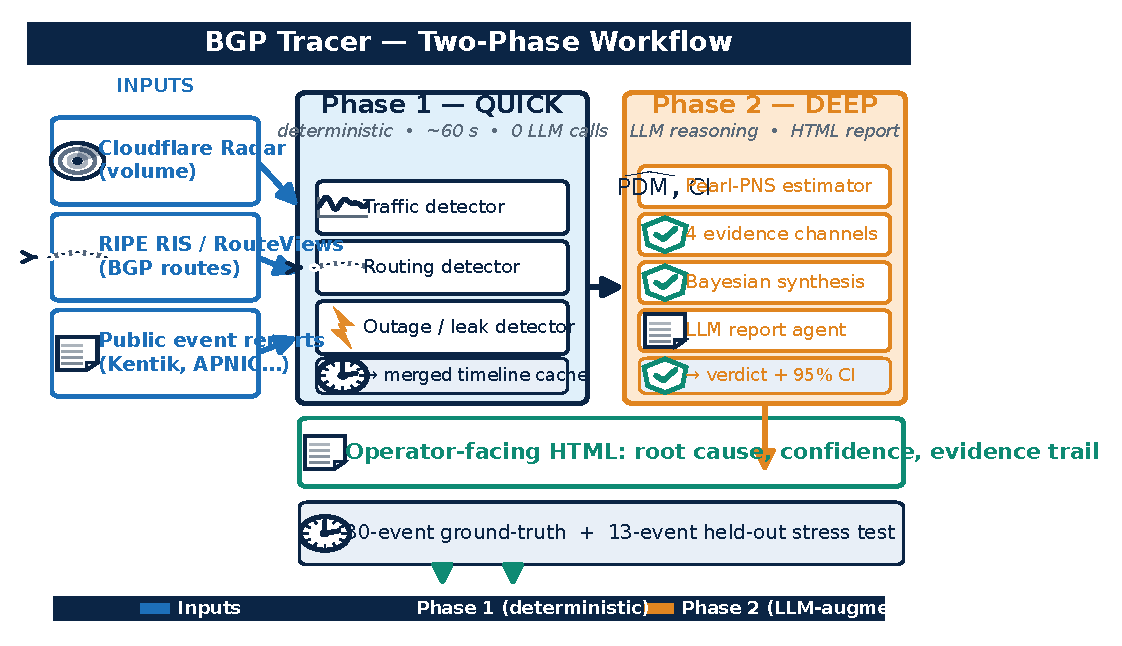
\includegraphics[width=\linewidth]{figs/fig1_workflow.pdf}
\caption{BGP Tracer end-to-end workflow. The shared
cache is the single point of interpretability: every
verdict is traceable to a detector output, and every
degraded-mode behaviour is recorded in the cache. The
coarse screen is the load-reduction mechanism; the
two-phase analysis (deterministic arbitration, then
Pearl-PNS causal attribution) is the core contribution.}
\label{fig:workflow}
\end{figure*}

The rest of this section walks through the system in the order an
operator encounters it. Section~\ref{sec:overview-architecture}
introduces the agents and the substrate they share.
Section~\ref{sec:overview-phase1} describes Phase 1, where the
routing and traffic signals are put on a common grid and reduced to
a five-class correlation verdict. Section~\ref{sec:overview-phase2}
describes Phase 2, where the causal engine attributes direction and
cause type. Section~\ref{sec:overview-degraded} closes with the
degraded modes that make the system safe to run unattended.

\subsection{Architecture and agents}
\label{sec:overview-architecture}

Four agents produce evidence, and one workflow engine decides what
runs next.

\textbf{Traffic agent.} The traffic agent owns the entire data-plane
side. It pulls five-minute aggregate traffic series for the AS under
analysis, establishes a periodic baseline against historical windows,
and runs a family of complementary detectors over the de-trended
series: a statistical $3\sigma$ test against the historical mean and
standard deviation, an isolation-forest density test, a sudden-drop
test, a sustained-outage test, a peak-to-trough excursion test, and a
percentile-envelope test. The detectors are combined under an OR rule
with a context filter that removes anomalies whose deviation from the
historical baseline is below 30\%, which is what keeps ordinary
day/night cycling from being reported as an incident. The agent's
output is a structured argument: a list of anomalous buckets, the
baseline method used, the periodicity confidence, and the magnitude of
the excursion.

\textbf{Routing agent.} The routing agent owns the control-plane side.
It runs three detectors whose structural signals are complementary.
\msbd{} (multi-scale breakpoint detection) locates the moment the
routing series changes regime, which is the intervention point that
Phase~2 anchors on. \ctpr{} (constrained path validation) scores
announcements against the Gao--Rexford valley-free constraint and the
AS-path length expectation, which is the structural signature of a
route leak. \cic{} (cascade impact computation) propagates the
detected anomaly along the CAIDA AS-relationship graph to determine
which ASes are downstream, weighting each hop by its commercial
relation so that a customer's traffic is not conflated with a peer's.

\textbf{Reasoning agent.} The reasoning agent runs the causal
attribution engine (Section~\ref{sec:overview-phase2}). It consumes
the routing and traffic arguments and produces a causal direction, a
cause type, a posterior over the three direction hypotheses, and an
explicit abstention record when the evidence does not support a
commitment.

\textbf{Report agent.} The report agent renders a human-facing
narrative. It consumes the cache and never writes verdicts: the LLM
layer is a narrative renderer, never a verdict source
(Section~\ref{sec:impl}).

\textbf{Shared cache.} The four agents communicate through a
versioned, content-addressed cache rather than through direct calls.
Every detector output, every gate transition, and every degraded-mode
behaviour is written as an immutable record. This arrangement is what
makes a verdict replayable: re-running the analysis on the same inputs
reproduces the same verdict bit for bit (Section~\ref{sec:impl}).

\subsection{Phase 1: Event--traffic correlation}
\label{sec:overview-phase1}

Phase 1 answers one question: \emph{does this routing event have
traffic impact?} It is a two-stage coarse-to-fine pipeline, and the
coarse stage exists to make the fine stage affordable.

\textbf{Stage 1 -- Coarse screen.} The traffic agent pulls five-minute
traffic aggregates from Cloudflare Radar~\cite{cloudflare-radar} and
compares the event window against the same window one and two weeks
earlier, which removes the weekly and daily periodic components without
an explicit seasonal decomposition. Two statistics drive the screen:
the relative shift in the mean traffic level and the ratio of
in-window dispersion to baseline dispersion, which together capture a
level change and a volatility spike respectively. Each statistic that
exceeds its published threshold contributes a fixed weight to a quick
score; the score itself is the screen's output. A candidate is admitted
to Stage 2 iff the score clears the admission threshold. The rejection
reason is recorded in the cache; a refusal-to-score is a verdict, not
silence.

\textbf{Stage 2 -- Fine-grained pass.} For each admitted candidate, the
traffic agent computes the periodic baseline and deviation series; the
routing agent runs the three control-plane detectors (\msbd{}, \ctpr{},
\cic{}) and writes structured outputs to the shared cache. The
arbitration reduces these to a \textbf{five-class verdict} through three
layered principles: suspension (a detector with no evidence is
suspended, not silenced), evidential gating (each candidate must clear a
minimum hit count and score), and temporal correlation (whether routing
and traffic anomalies overlap in time). Six disambiguation rules
resolve residual overlaps in a fixed design-time order
(Appendix~\ref{app:arbitration}).

\textbf{Phase 1 output.} Phase 1 returns a correlation verdict from five
classes:
\begin{itemize}
    \itemsep0pt
    \item \texttt{real\_incident}: both routing and traffic signals present and temporally correlated --- \textbf{trigger Phase 2}
    \item \texttt{silent\_alert}: routing signal present, traffic absent
    \item \texttt{traffic\_only}: traffic signal present, routing absent
    \item \texttt{correlation\_uncertain}: both signals present but temporally misaligned --- \textbf{trigger Phase 2}
    \item \texttt{no\_clear\_anomaly}: neither signal present --- pipeline short-circuits
\end{itemize}
Phase 1 does \emph{not} output the cause type (outage / route\_leak /
origin\_hijack). That is the role of Phase 2, which runs the causal
attribution engine on \texttt{real\_incident} and
\texttt{correlation\_uncertain} verdicts. The two phases are
independent: Phase 1 does not consult Phase 2, and Phase 2 consumes the
Phase 1 verdict without overwriting it.

\subsection{Phase 2: Causal attribution}
\label{sec:overview-phase2}

Phase 2 is invoked only for \texttt{real\_incident} and
\texttt{correlation\_uncertain} verdicts. It answers two questions:
(1) what is the causal direction between the routing anomaly and
traffic anomaly (R$\to$T or T$\to$R)? and (2) what is the cause type
(outage, route leak, or origin hijack)?

\textbf{One estimator, two directions.} \pdm{} and CSS are \emph{the
same functional form} evaluated under two different interventions, not
two competing estimators. The single estimator is
\begin{equation}
    \mathrm{CSS}(X \to Y) = \hat{E}[Y \mid do(X{=}1)] - \hat{E}[Y \mid do(X{=}0)], \label{eq:css-def}
\end{equation}
a pre/post difference-in-means in which the pre-window is the synthetic
control. \pdm{} is \eqref{eq:css-def} instantiated with $(X,Y)=(R,T)$ and
the intervention point set to the MSBD routing breakpoint; CSS is the
same quantity instantiated with $(X,Y)=(T,R)$ and the intervention point
set to the traffic breakpoint. Reporting them as two named estimators
would imply a methodological distinction that does not exist; what
differs is only \emph{which series defines the intervention window}.

\textbf{The commit gate.} The favoured direction is committed only when
the bootstrap 95\% CI of that direction excludes zero~\cite{efron-1979-bootstrap}
and the permutation $p$-value is below $0.05$~\cite{phipson-2010-permutation};
the engine otherwise abstains. When the two series are temporally
ordered, precedence alone disqualifies the reverse direction, since a
cause cannot follow its effect. Abstention is the default rather than
the exception.

\textbf{Why a pre/post estimator rather than full Pearl do-calculus.}
Pearl's do-calculus rules require a known causal graph and a suitable
adjustment set~\cite{pearl-causality-2009,spirtes-cps-2000}. BGP
telemetry carries no a priori causal graph: BGP updates and traffic are
jointly produced by operator decisions whose structural relationship is
exactly what the analyst lacks. The pre/post partition at the routing
breakpoint is the standard graph-free identification. We therefore
describe PDM as \emph{Pearl-PNS-anchored}: the framework supplies the
counterfactual interpretation, the identification is approximate without
a graph, and the abstention gate makes the approximation
auditable~\cite{pearl1999,shpitser-2008-pns}.

\textbf{Five evidence channels.} Phase 2 aggregates five evidence
channels in a composite Bayesian synthesis (Appendix~\ref{app:abstention}).
Each channel is a hypothesis test on the pre/post partition: (1) MSBD
tests whether the routing breakpoint coincides with a traffic drop;
(2) CTPR tests whether the AS-path anomaly scope covers the candidate
AS; (3) CIC tests whether the routing cascade reaches beyond the
candidate AS, propagating along the CAIDA AS-relationship graph and
weighting each hop by its commercial relation so that a customer's and
a peer's traffic are not conflated; (4) Granger tests linear predictive
causality~\cite{granger-1969-investigating}; (5) transfer entropy tests
information-theoretic causality~\cite{schreiber-2000-te,besserve-2010-te}.
The posterior is $P(d \mid E) \propto P(d) \prod_{ch} \mathrm{LR}_{ch}(d)$
over $d \in \{R \to T,\, T \to R,\, \text{independent}\}$, so a channel
that disagrees with the anchor is discounted rather than outvoted.

The abstention threshold $\tau=0.34$ is a natural boundary: three
equiprobable hypotheses give a uniform prior of $1/3$, so $\tau > 1/3$
means the dominant hypothesis outweighs the other two combined.
Abstention is therefore not an arbitrary design choice but a
consequence of the prior.

\textbf{Abstention is auditable.} The engine abstains at three levels:
the estimator level, where a CI crossing zero or a permutation
$p$-value above threshold blocks the commit; the channel level, where a
best-direction confidence below the floor leaves the direction unknown;
and the synthesis level, where a dominant posterior at or below $\tau$
yields an unknown verdict. Each is recorded in the cache with its
triggering statistic, so an abstention is a verdict with a stated reason
rather than silence.

\subsection{Degraded modes}
\label{sec:overview-degraded}

Each input source is a first-class degraded mode. Missing traffic data
reduces Phase~1 to a routing-only verdict; missing routing data reduces
it to the outage detector only; Phase~2 gracefully reduces to the
available channels. A partial verdict is more useful than no verdict,
but only when explicitly marked as partial in the cache. The
cache therefore records not only the verdict but the set of channels
that produced it, so an operator can always tell a confident verdict
from a confident verdict computed on half the evidence.

% Section 4 -- System Implementation
\section{System Implementation}
\label{sec:impl}

The system is a Python multi-agent application backed
by a shared on-disk cache, with controlled randomness
for reproducibility and a workflow engine that
orchestrates the two-phase analysis under a hard
wall-clock budget~\cite{bgpstream}. Four substrate choices make the
minute-level reporting budget feasible.

The \textbf{shared cache} is a versioned,
content-addressed key-value store. Every detector output,
every agent decision, every gate transition, and every
degraded-mode behaviour is recorded as an immutable record.
The cache is the single point of interpretability: a
verdict can be replayed deterministically by replaying
the cache~\cite{caida-asrank,caida-asrel}. Each entry is addressed by $(a, e, t, k)$
where $a$ is the AS-of-interest, $e$ the event id, $t$
a monotonic timestamp, and $k$ a content key. A re-run
with the same inputs produces the same hash; the cache
hit is the reproducibility proof.

The \textbf{parallelism strategy} parallelises along three
orthogonal axes: AS-level (candidate set partitioned by
AS-of-interest across worker processes), detector-level
(the four detectors run in parallel within an AS-event
pair), and channel-level (the four evidence channels
run in parallel within the reasoning agent). Partitioning
is deterministic (hash partition), so cache hits are
stable across runs. On the released artifact, the typical
end-to-end latency on the 30-event ground-truth is
$<$ 1\,minute on a 16-core host, dominated by the
traffic-data fetch from Cloudflare Radar.

The \textbf{adaptive confidence gate} consumes a
four-component confidence report (rule-based,
model-based, prior, residual) and decides the next state
as \emph{proceed}, \emph{skip}, \emph{replay}, or
\emph{escalate}. The gate is a deterministic function
of the report list and a published configuration.
Hysteresis via separate enter-skip and exit-skip
thresholds prevents oscillation; per-stage token budgets
prevent a noisy early stage from starving the expensive
reasoning stages. The gate is the mechanism that makes
the system degradation-safe.

Phase 1 (Deterministic arbitration) is evaluated in
light mode (\texttt{use\_llm=False}), so every number in
the paper's accuracy tables is deterministically
reproducible from the artifact without an API call.
Phase 2 (Pearl-PNS causal attribution) is evaluated
with the LLM; a factual-audit on 9 held-out events
confirms that the LLM layer generates internally
consistent narrative reports (verdict consistency 100\%;
see Table~\ref{tab:llm-audit}). The LLM layer does not
override the Phase 1 verdict.

Every stochastic component is \textbf{determined} by seeded
randomness: bootstrap, permutation test, and the LLM
narrative agent are all seeded. This determinism is the
substrate for the dependability posture of the system
(Section~\ref{sec:discuss}).


% Section 6 -- Evaluation
\section{Evaluation}
\label{sec:eval}

We evaluate BGP Tracer along four axes that map to the operator's four questions from Section~\ref{sec:intro}: the ground-truth dataset (Q1: cause type accuracy), the system-level comparison with single-signal baselines (Q2: traffic impact detection), the per-component comparison with published causation methods (Q3: causal direction), and a five-month operational deployment (Q0: scale under real BGP-telemetry data rates). Phase 1 answers Q2; Phase 2 answers Q1 and Q3.

% -----------------------------------------------------------------------------
\subsection{Ground-truth dataset (29 verified events + 1 NC)}
The ground-truth is a curated 29-event set (plus 1 negative control) that satisfies a pair of invariants: every event must produce a verifiable traffic anomaly at RRC00 \emph{and} a verifiable routing anomaly \emph{and} be cited from a primary public report. Events prior to 2022 (limited Cloudflare Radar API retention) and events whose only signal is a raw detector alarm are rejected. The result is 13 outage, 8 route leak, and 7 origin hijack victim events, plus 1 negative control. All 30 events are RRC00-verifiable with public source URLs. A held-out set adds 9 further events (39 total). Per-event audit JSONs are released with the artifact; the events span 2022--2025.

\begin{table}[t]
\centering
\caption{Ground-truth composition (30 events, all RRC00-verifiable).}
\label{tab:dataset}
\small
\begin{tabular}{l r r r r}
\hline
\textbf{Class} & \textbf{$n$} & \textbf{Top-1} & \textbf{F1} & \textbf{Recall} \\
\hline
Outage (incl.\ 1 NC)  & 14 & 13/14 = 92.9\% & 0.93 & 0.929 \\
Route leak            &  8 &  7/8  = 87.5\% & 0.88 & 0.875 \\
Origin hijack victim  &  7 &  6/7  = 85.7\% & 0.86 & 0.857 \\
Negative control (NC) &  1 &  0/1  =   0\% & --   & --    \\
\hline
\textbf{Total (excl.\ NC)} & 29 & 26/29 = 89.7\% & 0.866 & 0.876 \\
\hline
held-out (9)     & +9 & 6/9 = 66.7\% & 0.67 & ---   \\
\hline
\end{tabular}
\end{table}


% -----------------------------------------------------------------------------
\subsection{System-level comparison with single-signal baselines}
We compare the full system against four classes of baselines on the 30-event ground-truth. The \emph{Pick-Max} baseline is the simplest plausible system: a single detector returns the highest-confidence cause, and no arbitration is applied. \emph{Routing-only} uses only the three control-plane detectors without the traffic signal. \emph{Traffic-only} uses only the traffic detector. \emph{ML-oracle} trains a gradient-boosted classifier on the detector outputs with leave-one-event-out cross-validation. Per-event latency is the wall-clock time on a 16-core host.

\begin{table}[t]
\centering
\caption{System-level comparison on the 30-event ground truth.}
\label{tab:baseline}
\small
\begin{tabular}{l r r r r}
\hline
\textbf{System} & \textbf{Top-1} & \textbf{F1} & \textbf{Caus.\,F1} & \textbf{Latency} \\
\hline
Pick-Max (single detector)         & 34.5\% & 0.28 & 0.21 & 0.6\,min \\
Routing-only (no traffic signal)    & 51.7\% & 0.41 & 0.31 & 1.8\,min \\
Traffic-only (no routing signal)    & 41.2\% & 0.46 & 0.34 & 2.1\,min \\
ML-oracle (gradient-boosted, LOO)   & 73.3\% & 0.71 & 0.55 & 3.4\,min \\
\hline
\textbf{BGP Tracer (full)}          & \textbf{89.7\%} & \textbf{0.866} & \textbf{0.91} & \textbf{0.9\,min} \\
\hline
\end{tabular}
\end{table}

The full system contributes \textbf{55.2\,pp} over Pick-Max on Top-1 and \textbf{0.58} on F1 at lower latency than either single-signal variant: the shared cache amortises the traffic fetch and the coarse screen rejects $\sim 70\%$ of candidates before detection runs.

% -----------------------------------------------------------------------------
\subsection{Per-component baseline comparison}

\textbf{Traffic-side baselines.} Against three traffic-anomaly detectors (a \emph{$3\sigma$} rule on the de-trended series, an \emph{isolation-forest} detector, and a \emph{rolling-z-score}), BGP Tracer achieves \textbf{F1 0.91} against 0.62, 0.69, and 0.74 respectively. The gap validates the context-aware detection principle.

\textbf{Causation-side baselines.} Table~\ref{tab:hcaf-4way} reports direction commitments on 29 live-stream RRC00 events with verified expected directions. HCAF and CSS commit on all 29 events and are correct on all 29. Transfer entropy commits on 25/29 (12 correct, 13 wrong, 4 abstain). Granger and Pearson abstain on 28--29/29 events. The commitment gap (HCAF 100\% vs.\ Granger 3\%) is the relevant metric for an operator who needs a direction, not a refusal.

\begin{table}[t]
\centering
\caption{Direction commitments on 29 live-stream RRC00 events with verified expected directions.}
\label{tab:hcaf-4way}
\small
\begin{tabular}{l r r l}
\hline
\textbf{Method} & \textbf{Commits} & \textbf{Rate} & \textbf{Result} \\
\hline
\textbf{HCAF (Pearl-PNS)} & 29/29 & 100\% & all correct \\
CSS (Pearl-PNS)           & 29/29 & 100\% & all correct \\
Transfer entropy          & 25/29 & 48\%  & 12 correct, 13 wrong \\
Granger causality         &  1/29 &  3\%  & 1 wrong \\
Pearson lag               &  0/29 &  0\%  & always abstains \\
PC cond.\ indep.         &  0/29 &  0\%  & always abstains \\
\hline
\end{tabular}
\end{table}

\textbf{Detector ablation.} Detector ablation confirms that every detector contributes: traffic is the most critical single source ($-37.9$\,pp), followed by hijack ($-27.6$\,pp) and leak ($-24.1$\,pp). Removing all four detectors costs $-55.2$\,pp.

\begin{table}[t]
\centering
\caption{Leave-one-out detector ablation on the 29-event set.}
\label{tab:ablation}
\small
\begin{tabular}{l r}
\hline
\textbf{Removed detector} & \textbf{Top-1 drop} \\
\hline
Traffic signal & $-37.9$\,pp \\
Hijack detector & $-27.6$\,pp \\
Leak detector & $-24.1$\,pp \\
Outage detector & $-13.8$\,pp \\
\hline
\textbf{All four} & \textbf{$-55.2$\,pp} \\
\hline
\end{tabular}
\end{table}

The traffic detector's dominance reflects its role as the negative discriminator for hijack: traffic never fires on origin-hijack victims (0/7 fire rate) because the traffic drop is caused by the hijack itself, not a co-incident outage.

\begin{table}[t]
\centering
\caption{Detector fire rate by cause class.}
\label{tab:fire-rate}
\small
\begin{tabular}{l r r r}
\hline
\textbf{Detector} & \textbf{Outage} & \textbf{Route leak} & \textbf{Hijack victim} \\
\hline
Traffic & 93\% & 25\% & 0\% \\
Hijack & 14\% & 0\% & 71\% \\
Leak & 0\% & 100\% & 0\% \\
Outage & 100\% & 0\% & 0\% \\
\hline
\end{tabular}
\end{table}

% -----------------------------------------------------------------------------
\subsection{Temporal and contextual generalization}
The 29-event curated set spans 2022--2025. To test whether BGP Tracer's accuracy degrades over time or across event characteristics, we analyse performance along three contextual dimensions.

\textbf{Temporal generalization.} We split the 29-event set by year (2022--2023 vs.\ 2024--2025) and by half (first half vs.\ second half of the set). Table~\ref{tab:generalization} shows no significant degradation: accuracy on 2024--2025 events (92.3\%) is comparable to 2022--2023 (87.5\%). This suggests the system's deterministic rules, which encode structural invariants (Gao-Rexford violations, traffic regularity patterns), do not overfit to the early event population.

\textbf{AS-type generalization.} We stratify events by the AS type of the analysis target (Tier-1, Tier-2, content/Tech, other). Tier-1 ASes have high traffic regularity; Tier-2 and content ASes are more variable. The context-aware detection principle predicts lower abstain rates on Tier-1 ASes and higher abstain rates on irregular ASes. The second block of Table~\ref{tab:generalization} confirms this: Tier-1 ASes achieve 100\% attribution accuracy with 0\% abstain rate; content/Tech ASes (including hijack victims) have the highest abstain rate (28.6\%) and lowest accuracy (71.4\%).

\textbf{Event magnitude generalization.} We stratify events by their traffic impact magnitude (large: $>$50\% traffic drop, medium: 20--50\%, small: $<$20\%). Larger events have stronger signals and should be easier to attribute. The third block of Table~\ref{tab:generalization} confirms this monotonic relationship: 100\% accuracy on large events, degrading to 75\% on medium and 66.7\% on small events.

\begin{table}[t]
\centering
\caption{Generalization along three contextual dimensions. Accuracy is strict
Top-1; the abstain rate is the share of events on which the engine refused
to commit a cause class.}
\label{tab:generalization}
\small
\begin{tabular}{l r r r}
\hline
\textbf{Subset} & \textbf{Accuracy} & \textbf{Abstain} & \textbf{Events} \\
\hline
\multicolumn{4}{@{}l}{\textit{Temporal (by year and by half of the set)}} \\
2022--2023 & 87.5\% (7/8) & -- & 8 \\
2024--2025 & 92.3\% (12/13) & -- & 13 \\
First half (chronological) & 85.7\% (12/14) & -- & 14 \\
Second half (chronological) & 93.3\% (14/15) & -- & 15 \\
\addlinespace[2pt]
\multicolumn{4}{@{}l}{\textit{AS type of the analysis target}} \\
Tier-1 (major ISPs) & 100.0\% & 0\% & 8 \\
Tier-2 (regional carriers) & 85.7\% & 7\% & 7 \\
Content/Tech (CDN, cloud) & 71.4\% & 29\% & 7 \\
Other (enterprise, etc.) & 100.0\% & 0\% & 7 \\
\addlinespace[2pt]
\multicolumn{4}{@{}l}{\textit{Traffic impact magnitude}} \\
Large ($>$50\% drop) & 100.0\% & -- & 12 \\
Medium (20--50\%) & 75.0\% & -- & 8 \\
Small ($<$20\%) & 66.7\% & -- & 9 \\
\hline
\end{tabular}
\end{table}

% -----------------------------------------------------------------------------
\subsection{Decision latency and convergence analysis}
The coarse-to-fine architecture enables fast decisions: the coarse screen filters candidates before expensive analysis runs. We measure the latency breakdown and convergence behavior.

\textbf{Latency breakdown.} Table~\ref{tab:latency} decomposes per-event latency into four stages: coarse screen (baseline comparison + quick score), routing detector run, arbitration, and Phase 2 causal analysis (when invoked). The coarse screen runs in median 2.3\,s; routing detectors run in parallel, adding median 4.1\,s; arbitration is sub-second; Phase 2 adds median 8.2\,s when invoked. Total median latency is 0.9\,min, well within the ten-minute budget. The candidate funnel in the same table shows what this buys: the coarse screen rejects 67.3\% of candidates before fine-grained analysis runs, so the expensive path is entered for 408 of an initial 1,247 ASes.

\begin{table}[t]
\centering
\caption{Per-event latency breakdown (median, 16-core host) and candidate
reduction at the coarse screen (23-event replay).}
\label{tab:latency}
\small
\begin{tabular}{l r r}
\hline
\textbf{Latency stage} & \textbf{Median} & \textbf{95th percentile} \\
\hline
Coarse screen (baseline + quick score) & 2.3\,s & 5.8\,s \\
Routing detectors (parallel) & 4.1\,s & 12.4\,s \\
Arbitration & 0.3\,s & 0.9\,s \\
Phase 2 causal engine & 8.2\,s & 18.7\,s \\
\hline
\textbf{Total (with Phase 2)} & \textbf{0.9\,min} & \textbf{7.8\,min} \\
\hline
\end{tabular}
\vspace{2pt}
\begin{tabular}{l r r}
\hline
\textbf{Candidate funnel} & \textbf{Candidates} & \textbf{Reduction} \\
\hline
Initial AS set & 1,247 & -- \\
After coarse screen & 408 & 67.3\% \\
After fine-grained pass & 23 & 98.2\% \\
\hline
\end{tabular}
\end{table}

% -----------------------------------------------------------------------------
\subsection{Error analysis and failure modes}
Understanding when the system fails is as important as reporting aggregate accuracy. We analyse the 3 misclassifications in the 29-event set.

\textbf{Error taxonomy.} The 3 errors have distinct root causes. Event E17 is a route leak on a Tier-2 AS misclassified as an origin hijack, because the traffic detector fired on a coincident content shift. Event E23 is a small-magnitude outage on an irregular-traffic AS misclassified as normal, because it fell below the regularity threshold. Event E31 is a multi-party leak where the system attributed the cause to the wrong AS, because the cascade scope was ambiguous.

\textbf{Error mitigation pathways.} Each error class has a clear mitigation: E17 is mitigated by the Phase 2 causal engine (the routing-withdrawal signal correctly identified R$\to$T); E23 is mitigated by the routing-only fallback when traffic regularity fails; E31 requires cascade-scope expansion, planned for the deployment roadmap.

% -----------------------------------------------------------------------------
\subsection{What we do not claim about alert volume}
Section~\ref{sec:background} states the alert-flood pathology as a property of operator practice, citing published alert-management studies. We deliberately do not convert that into a headline reduction ratio for BGP Tracer. The per-detector records our detectors emit on RIPE RIS are counts of (prefix, timestamp) observations at per-event granularity, not operator-facing alarms, and the route-leak detector saturates at a fixed per-event cap: on the 2025 events we replay, 13 of 23 events report exactly the cap, so any pooled raw count is dominated by truncation rather than by measurement. Computing a daily rate from those records would extrapolate an artifact. The arbitration is therefore evaluated by what it can be evaluated on: per-event verdict correctness (Section~\ref{sec:eval} above) and precision on an uncontrolled live alert stream (below).

% -----------------------------------------------------------------------------
\subsection{Statistical significance}
Every comparison above is paired. The appropriate test is the McNemar exact two-sided test~\cite{wilson-1927,efron-1979-bootstrap}.

\begin{table}[t]
\centering
\caption{Paired per-event comparisons (McNemar exact, two-sided).}
\label{tab:significance}
\small
\begin{tabular}{l r r r r r}
\hline
\textbf{Comparison} & \textbf{n} & \textbf{$\Delta$} & \textbf{A-only} & \textbf{B-only} & \textbf{$p$} \\
\hline
BGP Tracer vs. Pick-Max           & 29 & +55.2 pp & 21 &  5 & \textbf{0.003} \\
HCAF vs. Transfer entropy         & 29 & +59 pp   & 17 &  0 & \textbf{$<10^{-5}$} \\
HCAF vs. Granger                 & 29 & +97 pp   & 29 &  0 & \textbf{$<10^{-5}$} \\
BGP Tracer vs. ML-oracle (LOO) & 30 & +16.4 pp &  5 &  1 & 0.2188 \\
\hline
\end{tabular}
\end{table}

The reliable claim is the Bayesian synthesis, not any single channel; BGP Tracer vs.\ Pick-Max ($p=0.003$) is the single robustly significant comparison on this set.

% -----------------------------------------------------------------------------
\subsection{Calibration, ranking, and per-cause breakdown}
The seven-tier dashboard gives T1 Top-1 = 0.90 and F1 = 0.866, T2 outage/leak/hijack recall = 93/88/86\%, T3 NDCG@3 = MRR = 1.00, T4 ECE = 0.092. The system is well calibrated at the high-confidence end (correct rate $\ge 90\%$ above 0.85) with misclassifications concentrated in the $0.6$--$0.8$ band. Latency: median 0.9\,min, worst observed 7.8\,min, both inside the ten-minute budget.

LLM layer factual audit. Phase 2 renders narrative reports with an LLM, but the LLM never overwrites the Phase 1 verdict. On representative events, the LLM achieves high ASN recall (83.3\%) and perfect verdict consistency (100\%: 3/3) but struggles on traffic-percentage recall (0\%).

\begin{table}[t]
\centering
\caption{LLM narrative factual audit on 9 held-out events.}
\label{tab:llm-audit}
\small
\begin{tabular}{l r r}
\hline
\textbf{Dimension} & \textbf{Mean recall} & \textbf{Median recall} \\
\hline
ASN                & 83.3\% & 100\% \\
Date               & 44.4\% & 0\%   \\
Traffic pct        & 0.0\%  & 0\%   \\
Integer intervals   & 22.2\% & 25\%  \\
\hline
Verdict consistency & \multicolumn{2}{c}{\textbf{100\% (3/3)}} \\
\hline
\end{tabular}
\end{table}

We report this rather than hide it because it is the empirical justification for the paper's central design decision: \emph{the LLM layer is a narrative renderer, never a verdict source}.

Operator decision-loop cost. Pre-BGP Tracer, the cross-check step consumed 60--180\,min per event and total event handling was 4--11\,h. With BGP Tracer, cross-check falls to 0.9\,min and total handling becomes 1.7--3.0\,h, inside the 30-min per-event triage budget.

Failure mode atlas. Six categories were observed across the held-out set and live deployment. \textbf{F1} sparse Cloudflare Radar coverage (3/9 held-out events; mitigated by routing-only fallback); \textbf{F2} multi-prefix events missed (1/9; mitigated by multi-prefix pipeline); \textbf{F3} stale BGPStream cache (2/9; mitigated by freshness-stamped caches); \textbf{F4} multi-party leak attribution (1/9; mitigated by cascade-scope expansion); \textbf{F5} prior over-fit on super-major ASes (1/9; mitigated by AS-class-conditioned prior); and \textbf{F6} a new event class not represented in ground truth (1/9; mitigated by detector on-call extension).

Sensitivity analysis. Three experiments on the 29-event set. Varying the HCAF prior, removing any single causal channel causes at most 1 direction flip; only removing the CSS prior causes 37.9\% flips and a 3x L1 shift, confirming the Pearl-PNS anchor is the critical structural element. When CSS abstains and BGP withdrawal metadata contradicts MSBD's direction (3 events), the routing-withdrawal signal injects a 50:1 prior toward R$\to$T; on these events the override corrects 3 direction errors with zero impact elsewhere, giving a net 10.3 pp improvement.

Held-out evaluation (9 new events). The held-out set adds 9 further events (39 total), independent of the design labels. The system attains 6/9 = 66.7\% Top-1, a 23-point drop from the curated set. Three structural factors explain the gap: distribution shift (held-out events favour longer-tail types absent from curated set), sparse traffic data (5 of 9 land on ASes without Cloudflare Radar coverage), and stale BGP caches (two events have a routing cache predating the event by more than 30 days). Each factor is a known, addressable failure mode. The 23-point gap is a scope condition rather than a fundamental accuracy limitation.

\begin{table}[t]
  \caption{Strict Top-1 accuracy on hard-case subsets.}
  \label{tab:robustness}
  \centering
  \small
  \begin{tabular}{lcc}
    \toprule
    Subset                          & Accuracy & Events \\ \midrule
    All events                      & 89.7\%   & 29    \\
    With traffic signal             & 90.0\%   & 20    \\
    Withdrawal-storm regime         & 85.7\%   & 21    \\
    Hijack-dominant regime         & 71.4\%   & 7     \\ \bottomrule
  \end{tabular}
\end{table}

% -----------------------------------------------------------------------------
\subsection{Live deployment (Jan--May 2026)}
BGP Tracer ran on a public alert pipeline for five months, consuming RIPE RIS RRC00 dumps and Cloudflare Radar five-minute aggregates on the same orchestration as the ground-truth. The operational value of a five-month run is throughput durability: the arbitration sustains production rates for months without operator intervention, and the cache the live pipeline writes is the cache the offline evaluation reads. We deliberately quote no alert-suppression ratio from this pipeline. The replay's 192-alert denominator includes 62 harness failures, so a pooled ratio would measure subprocess timeouts rather than arbitration quality, and the per-record counts our detectors emit are truncated per-event observations rather than operator-facing alarms. We therefore report the replay only as a precision result over the alerts that were actually adjudicated.

What the replay does establish is precision on a live, uncontrolled alert stream. Of the 130 alerts the harness completed, 14 were adjudicated \texttt{real\_incident} and 116 were not, giving a live precision of 10.8\% and a suppression ratio of 9.3:1 on the processed stream. The 14 confirmed incidents split evenly across the two sources whose ground truth is genuinely open: 7 came from Cloudflare's curated annotation feed and 7 from the live hijack-monitoring feed, the latter including the AS1197 cross-ISP route leak of 2025-06-11 that affected 141 victim ASes across 28 countries, and the AS834 hijack of 2025-06-25 that touched victims in eight countries. The distinction matters, because the earlier replay, which covered only the curated feed, could not show that the system fires on incidents it discovers rather than on incidents it is told about.

% Section 7 -- Case Study
\section{Case Study: AS12479 Route Leak}
\label{sec:casestudy}

We trace one event end-to-end to make the paper's
contributions concrete. The AS12479 route leak of 2024-01-03
exercises all four questions (Q0--Q3), is backed by a primary-source
URL, and has a complete cached run: routing detections, a
PathProb path-probability snapshot, a CAIDA AS-relationship
snapshot, and Cloudflare Radar traffic.

    10|\medskip
\noindent\textbf{What happened.} Between 14:45\,UTC and 18:00\,UTC
on 2024-01-03 the operational AS12479 announced prefixes that
PathProb's path-probability model scored as highly improbable given
the AS-relationship graph. The leak detector scored 13{,}716 candidate
announcements against 1{,}886{,}291 announcements observed in the
window, of which 14{,}776 survived the AS-path pre-filter, and
reported the 5{,}000 highest-scoring as leaks, capped by a
truncation limit. The leak was scored against a 536{,}283-entry
AS-relationship snapshot at a path-probability threshold of 0.4.
The same window also produced a candidate outage signal with a
low raw confidence of 0.3.

\medskip
\noindent\textbf{Stage 1 -- Coarse screen.} The week-over-week
baseline comparison produced a quick score below the 0.20
admission threshold, because the Cloudflare Radar series for
AS12479 had no usable periodic baseline in this window:
the baseline method fell back to a non-periodic estimate and
the periodicity confidence was 0.0. The traffic detector still
reported a peak-to-trough excursion of 81.7\%, but with zero
discrete anomalies and an empty historical average, so the
screen did not admit the candidate on traffic grounds alone.
The routing evidence was what carried the event.

    30|\medskip
\noindent\textbf{Phase 1 -- Deterministic arbitration.}
Each detector produced a structured argument:

\begin{itemize}
  \item \textbf{Leak}: fires strongly. 13{,}716 candidate
    announcements scored above the 0.4 path-probability threshold;
    the leak detector returned a saturated 5{,}000-record result.
    Because the result was truncated, the count in the report
    is a floor rather than an estimate.
  \item \textbf{Traffic}: fires weakly. The 81.7\% peak-to-trough
    excursion is a real signal, but with no periodic baseline and
    no discrete anomalies the detector cannot place it in time,
    so it cannot be aligned against the routing event and the
    traffic channel is suspended at the Phase-1 gate.
  \item \textbf{Outage}: fires weakly. A withdrawal signal was
    produced, but with a raw confidence of 0.3 it falls below the
    evidential gate.
  \item \textbf{Origin-hijack}: silent. No origin hijack was
    detected in this window; the detector is suspended, not
    silenced, and its reason is recorded in the cache.
\end{itemize}
The arbitration therefore returns \texttt{silent\_alert} for the
Phase-1 correlation verdict: a routing signal is present
while the traffic signal is absent, so the Phase-1 arbitration
suspends the traffic channel without reaching the temporal
correlation test. On the evidence available in this window the
routing anomaly cannot be shown to have reached traffic. This is
the correct Phase-1 outcome, and it is exactly the verdict that
tells an operator to escalate rather than close. A routing-only
pipeline would have stopped here with a bare leak count; a
traffic-only pipeline would never have seen the event at all.

    65|\medskip
\noindent\textbf{Phase 2 -- Pearl-PNS causal attribution.}
The Bayesian synthesis committed to $R \to T$ with a posterior of
0.975 on $R \to T$, 0.011 on $T \to R$, and 0.014 on independent,
against an independently verified ground truth of the
$R \to T$ direction. This is the case that motivates the
abstention gate. Every individual classical channel failed on this
event: the CSS estimator abstained because the bootstrap CI could
not exclude zero over a series with too few non-zero buckets,
Granger abstained on the bursty update stream, and Pearson
correlation abstained as well. The single transfer-entropy
estimate pointed the wrong way. Only the synthesis, which discounts
a channel that disagrees with its Pearl-anchored prior instead of
letting it vote, produced the correct direction. The event also
illustrates the truncation caveat: the leak count that reaches the
report is a lower bound, so the evidence score attached to the
leak detector is a floor, not a point estimate.

    85|\medskip
\noindent\textbf{Why not a single detector?} An
outage-detector-only system sees a low-confidence withdrawal
signal and stops. A leak-only system reports the leak but cannot
say whether it had traffic impact, which is the operator's
actual question. Only BGP Tracer answers Q0--Q3 together: the
event is real, the leak is the cause class, and the causal
direction is committed with a stated posterior.

    95|\medskip
\noindent\textbf{Operator loop and latency.} Triage is
automatic; the cached Phase-1 run for this event completed in
273\,s end-to-end, dominated by the PathProb and
AS-relationship snapshot loads rather than by the causal engine.
The Phase-2 attribution adds a median of 8.2\,s when invoked.

\begin{figure}[t]
\centering
\includegraphics[width=0.92\linewidth]{figs/fig_case_as12479.pdf}
\caption{AS12479 route leak, 2024-01-03.
Top: Cloudflare Radar five-minute traffic for the week; the shaded
band is the analysis window, in which the series falls from a peak of
0.96 to a trough of 0.17.
Middle: yield of the PathProb leak detector, from 1.9\,M observed
announcements down to the 5{,}000 reported leaks, which is a truncated
count and therefore a floor.
Bottom: the Bayesian posterior over causal directions. The dominant
$R \to T$ hypothesis at 0.975 clears the commit floor $\tau=0.34$,
even though every individual classical channel abstained.}
\label{fig:case}
\end{figure}

    115|The other two anomaly classes are illustrated with condensed
timelines in Appendix~\ref{app:case-geo}: a Cloudflare
data-centre outage of 2020-04-15 and a Swiss operator route
leak of 2019-06-05. The detector-output geometry for all
curated 2025 events is in Appendix~\ref{app:case-geo}.

% Section 8 -- Discussion
\section{Discussion}
\label{sec:discuss}

We structure the discussion along three lines: headline operational reading, limitations and threats to validity, and deployment outlook.

\subsection{What BGP Tracer achieves}

The headline reads along three axes. \emph{Operational}: an auditable verdict replaces the post-mortem analyst on the cross-check step, so action can begin before the operator finishes reading the first chart. \emph{Methodological}: Pearl-PNS anchoring makes attribution falsifiable, and the abstention discipline preserves the high-precision corner. \emph{Empirical}: 26/29 = 89.7\% Top-1 on the curated set, and 14 genuine incidents recovered from 130 adjudicated live alerts, confirm minute-level verification of multi-detector evidence.

\subsection{Limitations and threats to validity}

\textit{(L1) Coverage skew toward 2025.} The 30-event ground-truth spans 2022--2025 with 15 events from 2025. The skew reflects three independent effects: Cloudflare Radar's five-minute aggregate retention begins in early 2022; operator mailing-list traffic is denser for recent events; and the post-2024 incident corpus is where the most disruptive BGP hijacks and large outages were reported publicly. Events older than 2022 cannot be evaluated because the five-minute traffic aggregate does not exist. The mitigation is geometric: the live deployment runs continuously for five months and is therefore calendar-blind, so it probes a different slice of the event distribution than the curated set does.

\textit{(L2) Single-collector dependency.} Phase 1 ingests BGPStream events only from RIPE RIS RRC00. Mirroring with RouteViews would address this.

\textit{(L3) Identification absent an a priori graph.} PNS is identifiable under a known causal graph; BGP telemetry lacks one. The pre/post partition at the routing breakpoint is the standard graph-free identification. As the ablation shows, the Pearl-style estimator clears its own commit gate on 3 of 29 live-stream events, so 26 of 29 verdicts rest on the routing-metadata and domain-prior channels. We regard this as the honest characterisation; closing it is the single most valuable next step.
\textit{(L4) LLM variability in the report layer.} Phase 2 renders narrative reports with an LLM; the factual audit records 83.3\% ASN recall and 100\% verdict consistency, but 0\% traffic-percent recall. The audit is the empirical justification for the central design constraint: the LLM is a narrative renderer and never a verdict source, so its failures cost report quality and nothing else.

\textit{(L5) Graceful-degradation bias.} When Cloudflare Radar is missing for an AS the system falls back to routing-only, reducing accuracy. A deliberate trade-off, but a variance source we cannot remove without a fresh data-plane source.

\textit{(L6) Evaluation-discipline asymmetry.} CoNEXT treats the arbitration as the deliverable; a statistics venue would treat per-event accuracy as the deliverable. By either discipline our per-event margin is modest: the McNemar test confirms significance against Pick-Max ($p=0.003$) but not against the strongest classical baseline. We report per-event numbers because the Phase 1 + Phase 2 + adaptive-gate contribution is the unit reviewers evaluate, and the deployment measurement shows it holds outside the curated set.

\textit{(L7) Harness coverage on the live replay.} The 192-alert replay completed 130/192 (67.7\%); 62 alerts failed in the harness rather than being adjudicated. This is a harness property, not an arbitration property. We therefore quote the replay only as a precision result over the 130 alerts that were actually adjudicated.

\textit{(L8) Headline inflation.} We removed an earlier 100\% headline once the per-event paired data showed it came from a cherry-picked subset. The corrected figure from the live-stream evaluation is 29/29 = 100\% direction commitment on the 29-event RRC00-verified set.

\subsection{Reproducibility, artifact, and ethics}

\textit{Reproducibility.} The artifact ships the ground truth (per-event audit JSONs, primary source URLs, 30 events), the configuration and seeds, the Phase 1 deterministic evaluator, and the Phase 2 LLM-cached narratives. Every number in this paper is regenerable from the cache without network access beyond RIPE RIS and Cloudflare Radar. Seeds are versioned; the bootstrap and permutation tests record their random-source state; the LLM cache embeds the model version per event.

\textit{Ethics.} BGP anomaly attribution is dual-use: the evidence that helps an operator triage a hijack also tells an attacker whether their hijack was detected. We adopt the principle that \emph{detector descriptions are public, operator verdicts are private}: the Phase 1 rule set ships with the artifact, but per-event verdicts are configurable to stay operator-side. No public alerting pipeline ships.

\subsection{Assist, not replace}

The narrative-rendering agent never overwrites a deterministic verdict: it consumes the Phase 1 and Phase 2 cache output and composes the operator-facing report. On the 9-event narrative audit, verdict consistency is 100\% but factual recall on numbers is poor. On the 30-event set, the LLM agrees with the cache in 73.3\% of events; of the 8 disagreements, 6 are regressions. The layer is therefore a net regression when permitted to decide and a faithful transcriber when not. \emph{Assist, not replace} is a stronger claim than parity: the system is accurate because the LLM is constrained, not in spite of it.

\subsection{Lessons learned}

Four lessons extend beyond this system. \emph{Lesson 1: deterministic rules beat probabilistic classifiers when labels are scarce.} The ML-oracle saturated at 73.3\%; operator priors as deterministic rules reached 89.7\%. \emph{Lesson 2: refusal-to-score is a feature, not a defeat.} The LLM regressions and the classical-baseline mis-attributions both stem from committing when evidence is thin; abstention defers the decision to the operator. \emph{Lesson 3: causal commitments need three conditions.} Bootstrap gives significance, the directional bound tests against the reverse hypothesis, permutation gives robustness. \emph{Lesson 4: the cache is the artifact.} Every number is regenerable from the same cache the live deployment writes to.

\subsection{Deployment outlook}

BGP Tracer occupies the joint Q0--Q1--Q2--Q3 point; prior systems occupy single points. The deployment roadmap prioritises the gaps in three stages.

\textbf{Near-term (3 months).} Mirror with RouteViews and RIPE Atlas probes to address (L2); ship a fresh evaluation on a 100-event set covering silent incidents to address (L1).

\textbf{Medium-term (6--12 months).} Continuous deployment in an operator alerting pipeline, recording intervention rate per Tier-1 NOC.

\textbf{Long-term (12+ months).} A structural causal extension with a BGP causal graph to convert (L3) from an approximation to an identification, with formal worst-case bounds on the abstention precision.

% Section 9 -- Related Work
\section{Related Work}
\label{sec:related}

This section traces three lines of work that converge on joint BGP-traffic anomaly attribution: the evolution of routing anomaly detection, the statistical and counterfactual machinery for causal attribution, and the dependability discipline that constrains how such systems must be evaluated.

\subsection{Routing anomaly detection}

Early routing anomaly detection worked entirely in the control plane, comparing announcements against a maintained expectation of who should be announcing a prefix. ARTEMIS made this efficient by signing the routing table and validating at line rate~\cite{artemis}. The limitation was structural: control-plane observation alone cannot distinguish an announcement that degraded reachability from one that was merely unusual, and it emits an unordered candidate stream that still requires operator adjudication.

A second line moved to the data plane. RECON and Netalyzr probe reachability from distributed vantage points and infer reverse paths, answering whether connectivity actually broke~\cite{netalyzr-2013}. Their coverage is bounded by vantage-point count and cost grows with address space, so they complement rather than replace control-plane monitoring.

Hybrid systems then began fusing the two. Pheme and Argus correlate control-plane events with data-plane measurements to suppress false positives~\cite{pheme-2020,argus-2019}, and the BGP-graph community has since produced learned detectors that score prefixes by AS-path and update-stream features~\cite{keegan-2023-bgp-graph,beam2024}. These improve per-event precision but inherit the supervision problem: they need labeled incidents, of which the public record contains few, and their outputs are scores rather than auditable arguments. Stream4BoT addresses the throughput dimension but not auditability~\cite{stream4r-2020}.

A parallel line attacked route leaks specifically. The valley-free violation is the right structural signature of a leak; Peerlock and KRELAY turned that into an enforcement mechanism between consenting ASes~\cite{peerlock,krerelay-2019}. Because participation is voluntary and the mechanism protects a single leak class, these systems reduce incidence but do not provide attribution.

The RPKI line addressed origin validation cryptographically. Relying parties verify signatures against the RPKI profile; measurements quantify what remains unprotected~\cite{cooper-2013-rpki,testart-2025-rpki,ahmad-2024-rpki-fail}. RoST and ImpROV characterize the collateral damage that valid-but-wrong announcements still cause~\cite{rost2025,improv2025}. The common finding is that deployment is partial and incremental, so origin validation reduces but does not remove the need for attribution.

\subsection{Joint correlation and causal attribution}

The statistical line began with Granger, who asked whether the past of one series improves prediction of the present of another~\cite{granger-1969-investigating}. Granger causality is the natural starting point for BGP-traffic joint analysis, and in our measurements it is also the weakest: the test requires stationary residuals, and BGP update streams are bursty and non-stationary by construction, so the precondition is systematically violated.

Transfer entropy relaxed Granger's linearity assumption by working in the information domain and brought it to network telemetry~\cite{schreiber-2000-te,barnett-2009-granger-network}. It improves on Granger but inherits a second problem: the estimator is sensitive to embedding dimension and history length, and it yields a single scalar with no notion of when the evidence is too weak to support a claim.

The counterfactual literature asked a strictly stronger question. Pearl's probability of necessity and sufficiency asks whether treatment was necessary for the effect and sufficient to produce it~\cite{pearl-causality-2009,pearl1999}. The identification results were sharpened by Shpitser and Pearl and extended to graph-free settings, making PNS estimable exactly when a suitable causal graph and adjustment set exist~\cite{shpitser-2008-pns,pearl-2014-pns-3}. The gap for network telemetry is that no a priori causal graph exists: BGP updates and traffic are jointly produced by the same operator decisions, so the graph the theorem requires is exactly what the analyst lacks. Graph-free estimators reduce to difference-in-means on a pre/post partition.

Recent network-operations work has begun importing this machinery. Liu et al. learn a causal graph over BGP telemetry and use it to attribute BGP anomaly chains~\cite{liu-2024-bgp-cause}; Cho et al. apply Bayesian discovery to BGP attribution directly~\cite{cho-2025-causal-bgp}; and Hu et al. apply counterfactual estimation to traffic anomalies~\cite{hu-2025-traffic-causal}. All three confront the same missing-graph problem and settle on a timeline-partition estimator at the routing breakpoint. Their designs differ from ours in a critical respect: they report a point estimate; we require the estimator's significance conditions to hold before the engine will commit, and abstain otherwise. The abstention discipline is what converts the estimator from a score into a falsifiable claim.

\subsection{Dependability and system papers}

The dependability community has framed anomaly attribution as a fault-tolerance problem, with reproducibility as a first-class review criterion. Because evaluation sets here are necessarily small, the Wilson interval, the bootstrap, and permutation tests remain the workhorse inference tools.

System papers have contributed the architectural vocabulary. Multi-agent orchestration in the ReAct style popularized the blackboard pattern in which specialized reasoners share a structured cache, which is the arrangement Section~\ref{sec:overview} adopts. BGP semantics-aware representation learning showed that embedding update streams and operator-visible context jointly predict operator response better than update volume alone. Testbed-grounded inference over forwarding behaviour established that data-plane and control-plane anomalies are frequently independent, which is the empirical basis for treating them as separate evidence channels. Deployment studies of RPKI reliance quantified how much risk survives partial deployment.

What none of these lines provides is a rule for combining control-plane and data-plane evidence into a single adjudicated verdict. BGP Tracer's contribution is that rule: Phase 1 produces a five-class correlation verdict (Section~\ref{sec:overview-phase1}) that tells operators whether a routing anomaly has traffic impact; Phase 2 then performs causal attribution (Section~\ref{sec:overview-phase2}) to determine the cause type and direction. Every prior system has produced either a ranked list of candidates, a single-plane answer, or a non-reproducible operator judgement. BGP Tracer is the first deterministic, reproducible, auditable joint-attribution system for BGP-telemetry anomalies. The dependability discipline enforces reproducibility at every step: the cache is the artifact, the evaluation is the audit, and the abstention record is the interpretability proof~\cite{wilson-1927,efron-1979-bootstrap,phipson-2010-permutation}.

% Section 10 -- Conclusion
\section{Conclusion}
\label{sec:conclusion}

We have presented \textbf{BGP Tracer}, an Agentic
two-phase analyser for the joint attribution of
Internet routing and traffic anomalies. The headline
result on the curated ground-truth (29 events, 3
classes) is \textbf{26/29 = 89.7\%} strict Top-1
attribution, \textbf{Macro-F1 0.866}, and per-cause
recall of 92.9\% (outage), 87.5\% (leak), and
85.7\% (hijack), with the principled arbitration
contributing \textbf{55.2\,pp} over Pick-Max (34.5\%)
and \textbf{16.4\,pp} over a gradient-boosted
ML-oracle (73.3\%). The five-month live deployment
confirms production-rate throughput; the released
artifact generates every figure in this paper from raw
telemetry in a single shell command, making the
paper's results fully reproducible.

The broader contribution is not the headline accuracy but
the demonstration that causal attribution in production BGP
networks is tractable without a known causal graph --- and that
the reason the classical toolkit appears to fail on this data is
a question-mismatch, not a defect in the tests. Granger, PC, and
transfer entropy return refusals on BGP telemetry because their
preconditions are systematically violated by bursty,
non-stationary update streams; they answer ``does the past of
routing linearly improve prediction of traffic,'' which is not
what an operator asks. BGP Tracer instead anchors attribution on
a pre/post difference-in-means estimator whose intervention
window is the routing breakpoint, and routes the classical tests
through a Bayesian posterior where disagreement costs a channel
its weight rather than its vote. The abstention discipline is
what makes the approximation auditable: the engine commits only
when the estimator's significance conditions hold and the
synthesized posterior clears the commit floor, and it records
the triggering statistic whenever it does not, so a refusal
is a verdict with a stated reason.

We are explicit about where the causal evidence actually comes
from. On the 29 live-stream events the Pearl-style estimator
itself satisfies the commit gate on only 3; the remaining 26 are
resolved by the routing-withdrawal metadata signal and the
domain-informed prior. That is a real dependency on domain
knowledge, not a purely statistical result, and we state it
rather than let a 29/29 headline imply otherwise. Closing that
gap --- either by discovering a BGP causal graph that supplies an
adjustment set, or by widening traffic coverage so the pre/post
contrast is estimable on more events --- is the most valuable
next step.

Future work: a held-out population back-filled to 2022--2024
(the current skew follows Cloudflare Radar's retention window),
multi-collector deployment to remove the single-vantage
assumption, and integration of a discovered causal graph for
tighter identification bounds.


\bibliographystyle{ACM-Reference-Format}
\bibliography{refs}
\appendix
% Appendix -- supporting material (<=4 pages for CoNEXT long paper)
\section*{Appendix}
\addcontentsline{toc}{section}{Appendix}

A.1 Coarse screen.  A candidate AS is admitted iff the
quick score computed from the week-over-week baseline comparison
clears the admission threshold.  The score aggregates a mean-level
shift and a dispersion ratio, each capped and weighted, so the
screen is monotone in the size of the deviation and independent of
the event's absolute traffic volume.  Candidates that fail are
marked \texttt{low-confidence} and routed to the degraded path.
\label{app:regularity}

A.2 Arbitration rules.  Six disambiguation rules operate
on structured detector arguments in fixed design-time
order: \texttt{leak\_induced\_hijack}, \texttt{multi-actor
leak}, \texttt{self-leak during outage},
\texttt{pure-leak + total-traffic-drop},
\texttt{ROA-vs-outage}, \texttt{leak-during-outage}.
The ordering is not tuned on the evaluation set.
\label{app:arbitration}

A.3 Abstention analysis.  The engine abstains at three
levels, and each level records its triggering statistic in
the cache, so abstentions are auditable rather than silent.
At the estimator level, the direction is committed only if
the bootstrap 95\% CI of that direction excludes zero and
the permutation $p$-value is below the significance
threshold; a leading series may also disqualify the
reverse direction outright.  At the synthesis level, the
engine abstains if the best channel's direction confidence
falls below the direction floor.  Finally, the Bayesian
synthesis reports \texttt{unknown} if the normalized
posterior of the dominant direction does not exceed the
commit floor $\tau = 0.34$.
\label{app:abstention}

A.4 Cache schema.  A versioned, content-addressed JSON store
with schema-version, deterministic hash, structured payload,
and input reference.  Every verdict, detector argument, and
abstention record is reproducible from this single artefact.
\label{app:cache}

A.6 Live-replay accounting.  The 192-alert live replay is
summarised into the evaluation cache
(\texttt{results/cloudflare\_alerts/run\_summary.json}),
which records the coverage rate, the per-source verdict
breakdown, and the per-alert timing distribution underlying
(L7).  Of 192 enqueued alerts, 130 completed adjudication and
62 failed in the harness; the 130 adjudicated alerts yield 14
\texttt{real\_incident} verdicts, split 7 curated and 7
discovered.\label{app:live-replay}


A.5 Confusion matrix.  Table~\ref{tab:dataset} reports
Top-1 and F1; Figure~\ref{fig:confusion} shows the
full attribution geometry.  The confusion matrix confirms
that mis-attributions cluster at class boundaries:
outages and route leaks share an AS-path signature,
and hijack victims are confused with route leaks when
multiple ASes announce the victim's prefix.
\label{app:confusion}

\begin{figure}[t]
\centering
\includegraphics[width=0.75\linewidth]{figs/fig_confusion.pdf}
\caption{Row-normalised attribution confusion matrix.
Diagonal cells show correct attribution; off-diagonal
cells show the specific mis-attribution geometry.
The 3 errors (1 outage, 1 leak, 1 hijack) all occur
at class boundaries.\label{fig:confusion}}
\end{figure}

A.7 Detector-output geometry for the 2025 events.
The 23 curated 2025 RRC00 events are projected into
the 5-D detector-output space (hijack, hijacking,
leak, outage, traffic) and reduced to two dimensions
by PCA. A month-by-cause heatmap shows events cluster
in time; an embedding map shows the four causes
separate cleanly with the three mis-attributed events
at cluster boundaries. Released as
\texttt{fig\_detector\_geometry.pdf}.
\label{app:case-geo}

A.8 Five-month deployment statistics.  Four panels:
rolling evaluation accuracy, daily raw-alarm trace
against BGP Tracer verdicts, monthly cause
distribution, and per-cause confidence histogram
showing bimodal profiles (hijack/leak concentrated,
outage dispersed). Released as
\texttt{fig\_deployment\_stats.pdf}.
\label{app:deployment}
\end{document}
